\documentclass[acmsmall,screen]{acmart}
  \citestyle{acmauthoryear}
\usepackage{ amssymb }
  % \documentclass[acmsmall,10pt]{acmart}\settopmatter{printfolios=true} % ,review
% \citestyle{acmauthoryear}
\usepackage{subcaption}
\usepackage[T1]{fontenc}
\usepackage[utf8]{inputenc}
\usepackage[british]{babel}
\usepackage{xspace, listings, lstcustom, wrapfig, graphicx, enumerate}
\usepackage{paralist}
\usepackage{color, colortbl, relsize}
\usepackage{rotating}
\usepackage{pifont}
\usepackage{multirow}
\usepackage{soul}
\usepackage{tcolorbox}
\usepackage[scaled=.9, light]{zlmtt}
\usepackage{siunitx}
\usepackage{setspace}

   \newcommand{\ttt}{\prg{true}}
\newcommand{\ff}{\prg{false}}
\newcommand{\unkn}{\prg{b???}}
\newcommand{\bv}{\prg{bval}}


\newcommand{\prg}[1]{{\mbox{\tt{#1}}}}

\newcommand{\m}{\prg{m}}
 \newcommand{\f}{\prg{f}}
 \renewcommand{\c}{\prg{C}}
 \renewcommand{\v}{\prg{v}}
  \newcommand{\x}{\prg{x}}
  \newcommand{\p}{\prg{p}}
   \newcommand{\y}{\prg{y}}
  %  \newcommand{\z}{\prg{z}}
  \newcommand{\this}{\prg{this}}
  \newcommand{\caller}{\kw{caller}}
   \newcommand{\nullK}{\prg{null}}
\newcommand{\addr}{\ensuremath{\alpha}}
 
 \newcommand{\forget}[1]{}
\newcommand{\etc}{{\it etc.}}
\newcommand{\eg}{{\it e.g.\,}}
\newcommand{\ie}{{\it i.e.\,}}

\newcommand{\Future}[1] {{{\mathcal W}\!ill}(#1)}%{\lozenge\, #1}% {\bullet #1}% {{{\mathcal F}}(#1)} % {{{\mathcal B}}(#1)}
\newcommand{\Using}[2]{#1\,\kwN{in}\, #2} %{{{\mathcal U}}(#1,#2)}
\newcommand{\SigmaUsing}[2]{#1\@ #2} %{{{\mathcal U}}(#1,#2)}
\newcommand{\Past}[1] {{{\mathcal W}\!as}(#1)}% {\nabla #1} %{\lozenge\!\!\!\!\-\!\!-\,#1}
%{\lozenge\!\!\!\!\!\circ  #1} % {\lozenge\!\!\!\!\-\!\!- #1} %{\upupsilon #1}  %{\nabla #1} %{\circ #1}%  {{{\mathcal P}}(#1)}
\newcommand{\Initial}[1] {{{\mathcal I}\!nitial}(#1)}

\newcommand{\Pol}[1] {{\ensuremath{\prg{Pol}\_{\prg{#1}}}}}
 
\newcommand{\strongImplies}{\leqq} %{{ \,^\sqsubset\!\!\!_{\sim}\, }}
\newcommand{\weakImplies}{\lessapprox} %{{ \,^\sqsubset\!\!\!_{\sim}\, }}
\newcommand{\frames}{~\kw{frames}~}

\newcommand{\appref}[1]{see App.~\ref{#1}}

\newcommand{\sE}{{\prg{e}}}

\newcommand{\Lang} {\ensuremath{{\mathcal L}{_1}}}
\newcommand{\LangOO} {\ensuremath{{\mathcal L}{_{\tt {oo}}}}\xspace}

% ------------------------------------------------------------------
%                                             positions, separations
\newcommand{\cf}{{\it c.f.~}}
\newcommand{\HYPHENA}{{\em-- }}
\newcommand{\HYPHENB}{{\em-- }}
\newcommand{\SP}{{\hspace{.1in}}}
\newcommand{\s}{{\hspace{.01in}}}

\newcommand{\obeys}{\,\textbf{\textrm{obeys}}\,}
\newcommand{\StrongDom}{\ensuremath{\mathcal{S}\textrm{\textit{trong}}{\mathcal{D}}\textrm{\textit{om}}}}
\newcommand{\Dom}{\ensuremath{\mathcal{D}}\textrm{\textit{om}}}

\newcommand{\Changes}[1]{\ensuremath{\mathcal{C}\textrm{\textit{hanges}}(#1)}}
\newcommand{\VisibleLit}{\ensuremath{\mathcal{V}\textrm{\textit{isible}}}}

\newcommand{\Gives}{\ensuremath{\mathcal{G}\textrm{\textit{ives}}}}
\newcommand{\MayCall}{\ensuremath{\mathcal{M}\textrm{\textit{ay}}{\mathcal{C}}\textrm{\textit{all}}}}
%\newcommand{\Dom}{\ensuremath{\mathcal{D}\textrm{\textit{om}}}}
\newcommand{\MayRead}{\ensuremath{\mathcal{M}\textrm{\textit{ay}}{\mathcal{R}}\textrm{\textit{ead}}}}
\newcommand{\MayAccess}{\ensuremath{\mathcal{M}\textrm{\textit{ay}}{\mathcal{A}}\textrm{\textit{ccess}}}}
\newcommand{\CanAccess}[2]{\ensuremath{{\mathcal{A}}\textrm{\textit{ccess}}}(#1,#2)}
\newcommand{\Calls}[1]{\ensuremath{{\mathcal{C}}\textrm{\textit{alls}}}(\prg{#1})}
\newcommand{\Caller}{\ensuremath{{\mathcal{C}}\textrm{\textit{aller}}}}
%{\ensuremath{\mathcal{C}\textrm{\textit{an}}{\mathcal{A}}\textrm{\textit{ccess}}}(#1,#2)}
\newcommand{\WillAccessThrough}{\ensuremath{\mathcal{W}\textrm{\textit{ill}}{\mathcal{A}}\textrm{\textit{ccess}}{\mathcal{T}}\!\!\textrm{\textit{hrough}}}}
\newcommand{\modelsWithO}{\models\!\!\!\!{_{_{_{\tiny{\mathcal O}}}}}}
\newcommand{\A}{\ensuremath{A}}
\newcommand{\B}{\ensuremath{B}}
\newcommand{\Arising}[1]{{\mathcal{A}}\textrm{\textit{rising}}(#1)}

 %------------------------ syntax tables

\newcommand{\syntax}[1]{\prg{{\it #1}}}
\newcommand{\BBC}{$::=$} %in syntactic definitions
\newcommand{\SOR}{\ensuremath{\ \mid\ }} % BNF or
\newcommand{\MID}{{\SPsmall ~ \mid ~ \SPsmall }} % in sets


\newcommand{\pre}{\ensuremath{_{{pre}}}}   %kjx no \sc  in math mode
\newcommand{\post}{\ensuremath{_{{post}}}} %kjx no \sc  in math mode
\newcommand{\PRE}{\pre}
\newcommand{\POST}{\post}

 \newcommand{\interp}[2]{{\ensuremath{\lfloor{ {#1}}\rfloor_{#2}}}}
% \newcommand{\interpBL}[1]{{\lceil   {#1}  \rfloor}}
 
% ------------------------------------------------------------------
%                                              keywords, program text
\newcommand{\kw}[1]{\prg{#1}} % {{\bf{\sf {#1}}}}
\newcommand{\kwN}[1]{{\bf{\sf {#1}}}}
\newcommand{\returnKW}{{\bf{\sf {return}}}}
\newcommand{\newKW}{\mbox{\bf{\sf{new}}}}

\newcommand{\lit}[1]{{\prg {#1}\xspace}}
\newcommand{\com}{\ensuremath{\prg{//}}}
 
  
\newcommand{\ass}{\mbox{{\kw {:=}}\,}}
\newcommand{\semi}{\mbox{{\kw {;}}\ }}
\newcommand{\comma}{\mbox{{\kw {,}}\,}}
\newcommand{\lb}{\prg{\mbox{\tt{\bf{\{ }}}}}
\newcommand{\rb}{\prg{\mbox{\tt{\bf{\} }}}}}
\newcommand{\lp}{\prg{\mbox{\tt{\bf{( }}}}}
\newcommand{\rp}{\prg{\mbox{\tt{\bf{) }}}}}
%\newcommand{\thisL}{{\lit {this}}}% no~around it
\newcommand{\nullKW}{{\lit {null}}~}
\newcommand{\true}{{\lit {true}}~}
\newcommand{\false}{{\lit {false}}~}
\newcommand{\return}{{\kw {return}}\s}

 \newcommand{\M}{\prg{\ensuremath{\prg{M}}}}
  \newcommand{\Prog}[1]{\M{#1}}
  
\newcommand{\mkpair}{\fatsemi}
\newcommand{\subconf}{\ensuremath{\sqsubseteq}}
\newcommand{\restrct}[2]{\ensuremath{#1\!\!\downarrow\!_{#2}}}
\newcommand{\adapt}{\ensuremath{\!\triangleleft\!}}
\newcommand{\link}{\!\circ\!}

\newcommand{\ClassOf}[2] {\ensuremath{{\mathcal C}{\mathit{lass}}(#1)_{#2}}}

% --- assertions and expressions - simple
  
\newcommand{\SA}{\ensuremath{B}}%{\ensuremath{\prg{B}}} 
\newcommand{\SAPrime}{\ensuremath{B'}}

\newcommand{\SE}{\ensuremath{\prg{e}}}  
\newcommand{\SEPrime}{\ensuremath{\prg{e}'}}     
\newcommand{\SEOne}{\ensuremath{\prg{e}_1}} 
\newcommand{\SETwo}{\ensuremath{\prg{e}_2}}  


 

%\newcommand{\Prog}[1]  {{\ensuremath{\prg{M}{{\prg{#1}}}}}}
    % {\prg{P}}
 
\newcommand{\expandexp}[1]{}

\newcommand{\oo}{object-oriented}
\newcommand{\mExtS}{\ensuremath{\Downarrow}}

% re-classification expression
\newcommand{\cm}[1]{\this{\prg{\ensuremath{\mExtS}}}\prg{#1}}

\newcommand{\refDef}[1]{Defintion \ref{{#1}}}
  
% structuring macros
\newcommand{\EndDefLemma}{\noindent $\bigtriangleup$}

 %-------------------- implies, and, or, iff, etc -----------------
  \newcommand{\AND}{{\SPsmall {\mbox{and}} \SPsmall}}
\newcommand{\WITH}{{\SPsmall {\mbox{with}} \SPsmall}}
 \newcommand{\IFF}{{\SP {\mbox{ if }} \SP}}
\newcommand{\OR}{{\SPsmall {\mbox{or}} \SPsmall}}
\renewcommand{\implies}{{\ensuremath{\longrightarrow}}}
\newcommand{\upd}{{\mapsto}}

 






%Macros for inference rules
\newcommand{\inferencerule}[2]{
\begin{array}{l} #1 \\ \hline #2 \end{array}
}

\newcommand{\inferenceruleN}[3]
{
\begin{array}{l}
% \SP\SP\SP\SP\SP\SP\SP\SP
% \SP\SP\SP\SP\SP\SP\SP\SP
\SP\SP\SP\SP\SP\SP\SP\SP
\SP\SP\SP\SP\SP\SP  {\sf #1}
\\ #2  \\ \hline   #3
  \end{array}
}

\newcommand{\inferenceruleNN}[3]
{
\begin{array}{l}
\SP\SP\SP\SP\SP\SP\SP\SP
\SP\SP\SP\SP\SP\SP\SP\SP
\SP\SP\SP\SP\SP\SP\SP\SP
\SP\SP\SP\SP\SP\SP\SP\SP

   {\sf #1}
\\ #2  \\ \hline   #3
  \end{array}
}

%===========================================================================
%  Definition-Lemma-Theorem-Proof
%
% Adaptation of LaTeX's theorem environment; can be used as a command
% (eg just \Lemma not \begin{Lemma}) and no italicisation; also works
% with ptmac; result numbering is uniform within subsections and can be
% suppressed.
%
\newif\ifNumberResults\NumberResultstrue
\def\@@opargbegintheorem#1#2#3{\@@@@begintheorem{\bf\@@thmname{#1}{#2}(#3)}}
\def\@@begintheorem#1#2{\@@@@begintheorem{\bf\@@thmname{#1}{#2}}}
\def\@@@@begintheorem#1{\par\removelastskip\smallskip\noindent{#1}}
\def\@@thmname#1#2{#1\ \ifNumberResults#2\ \fi}

% similarly \Proof or \begin{Proof}...\end{Proof}
% prefer proofs with statements if possible - hence \penalty700
%\let\qedsymbol\S% make it \square or \blacksquare if you like for kb
\let\qedsymbol \Box
\def\qed{\hfill{$\qedsymbol$}}
\def\Proof{\par\removelastskip\smallskip\penalty700\noindent{\bf Proof}\enskip}
\def\endProof{\qed\penalty-700 \smallskip}
\let\endproof\endProof

%   The actual words

\newtheorem{theo}{Theorem}
 \newtheorem{definition}[theo]{Definition}
\newtheorem{example}[theo]{Example}
\newtheorem{mylemma}[theo]{Lemma}
\newtheorem{conjecture}[theo]{Conjecture}
% \newtheorem{theorem}{Theorem}
 \newtheorem{note}[theo]{Note}
 \newtheorem{observation}[theo]{Observation}


%--------------------------------- the ones that Susan introduced
\newcommand{\z}{{\prg z}}

\newcommand{\Fields}[3]{\ensuremath{{\mathcal F}(}\Prog{#1},\prg{#2},
\prg{#3}\ensuremath{)} }
\newcommand{\FieldIds}[2]{\ensuremath{{\mathcal F}{\it {s}}(\Prog{#1},\prg{#2})}}
\newcommand{\Meths}[3]{\ensuremath{{\mathcal M}(}\Prog{#1},\prg{#2},
\prg{#3}\ensuremath{)} }



 

\newcommand{\WideFig}[3]
{
\begin{figure*}[t]
\begin{center}
\noindent
\fbox{
\begin{minipage}{4.7 in}
{#1} % the contents
\end{minipage}
}
\caption{#2}
\label{#3}
\end{center}
\end{figure*}
}


\newcommand{\WideFigWhere}[4] % you can specify where it should appear!
{
\begin{figure*}[{#4}]
\begin{center}
\noindent
\fbox{
\begin{minipage}{5. in}
{#1} % the contents
\end{minipage}
}
\caption{#2}
\label{#3}
\end{center}
\end{figure*}
}

\newcommand{\BigWideFigWhere}[4] % you can specify where it should appear!
{
\begin{figure*}[{#4}]
\begin{center}
\noindent
{\normalsize
\hrule
\begin{minipage}{5. in}
{#1} % the contents
\end{minipage}
\hrule
}
\caption{#2}
\label{#3}
\end{center}
\end{figure*}
}

\newcommand{\NotTooWideFigWhere}[4] % you can specify where it should appear!
{
\begin{figure*}[{#4}]
\begin{center}
\noindent
\fbox{
\begin{minipage}{4.3 in}
{#1} % the contents
\end{minipage}
}
\caption{#2}
\label{#3}
\end{center}
\end{figure*}
}


\newcommand{\opsemExprFig}
{\BigWideFigWhere {\opsemExpr} {Execution of expressions\MD}
{opsemTrad} {htbp} }



\newcommand{\mlc}{ }%{\heartsuit}
%\newcommand{\mcl}{ }%{\heartsuit}
\newcommand{\mc}{ }%{\heartsuit}

\newcommand{\BigNotTooWideFigWhere}[4] % you can specify where it should appear!
{
\begin{figure*}[{#4}]
\begin{center}
\noindent
{\normalsize
\hrule
\begin{minipage}{4.3 in}
{#1} % the contents
\end{minipage}
\hrule
}
\caption{#2}
\label{#3}
\end{center}
\end{figure*}
}

 

%]})
%}


% \setcopyright{rightsretained}
%\acmPrice{}
%\acmDOI{10.1145/3133896}
%\acmYear{2018}
%\copyrightyear{2018}
%\acmJournal{PACMPL}
%\acmVolume{1}
%\acmNumber{????}
%\acmArticle{72}
%\acmMonth{10}
%
%\citestyle{acmauthoryear}
%
%
%
%\copyrightyear{2017}
%\copyrightdata{978-1-nnnn-nnnn-n/yy/mm}
%\doi{nnnnnnn.nnnnnnn}



%\usepackage[usenames]{color}

\usepackage{times}
 \usepackage{latexsym}
\usepackage{listings}
\definecolor{dkgreen}{rgb}{0,0.6,0}
\definecolor{gray}{rgb}{0.5,0.5,0.5}
\definecolor{mauve}{rgb}{0.58,0,0.82}


\lstset{ %
  language=Java,                % the language of the code
  mathescape=true,
  basicstyle=\footnotesize\tt,           % the size of the fonts that are used for the code
  numbers=left,                   % where to put the line-numbers
  numberstyle=\tiny\color{dkgreen},  % the style that is used for the line-numbers
  stepnumber=1,                   % the step between two line-numbers. If it's 1, each line
                                  % will be numbered
  numbersep=5pt,                  % how far the line-numbers are from the code
  backgroundcolor=\color{white},      % choose the background color. You must add \usepackage{color}
  showspaces=false,               % show spaces adding particular underscores
  showstringspaces=false,         % underline spaces within strings
  showtabs=false,                 % show tabs within strings adding particular underscores
  frame=single,                   % adds a frame around the code
  rulecolor=\color{black},        % if not set, the frame-color may be changed on line-breaks within not-black text (e.g. commens (green here))
  tabsize=2,                      % sets default tabsize to 2 spaces
  captionpos=b,                   % sets the caption-position to bottom
  breaklines=true,                % sets automatic line breaking
  breakatwhitespace=false,        % sets if automatic breaks should only happen at whitespace
  title=\lstname,                   % show the filename of files included with \lstinputlisting;
                                  % also try caption instead of title
  keywordstyle=\color{blue},          % keyword style
  commentstyle=\color{gray},       % comment style
  stringstyle=\color{mauve},         % string literal style
  escapeinside={\%*}{*)},            % if you want to add LaTeX within your code
  morekeywords={private,then,elseif,public,final,this,throw,new,||,to,def,any,fun,fld,abstract,policy,specification,ghost,field}        
         % if you want to add more keywords to the set
}

% \newcommand{\scd}[1]{{\color{blue}{#1}}}
% \newcommand{\jn}[1]{{\color{green}{#1}}}
% \newcommand{\sd}[1]{{\color{dkgreen}{#1}}}
% \newcommand{\sd}[1]{{{#1}}}

\begin{document}

%\preprintfooter{internal memo}

\author{ author1}\affiliation{ContinentOne}
 
%\authorinfo{Sophia Drossopoulou$^1$, James Noble$^{2,1}$, Toby Murray$^4$, Mark Miller$^3$, Shupeng Loh$^1$, Susan Eisenbach$^1$}{$^1$Imperial College London, $^2$Victoria University Wellington, $^3$Google Inc, $^3$NICTA and UNSW.}{}


\title{Holistic Specifications for Robustness} 


\begin{abstract}
\note{We need to make a better connection with work on safety. And why it is not sufficient.}


Functional specifications of program components describe what
components \emph{can} do --- the \emph{sufficient} conditions to
invoke the component's behaviour: a client who supplies arguments
meeting an operation's preconditions can invoke that operation. While
functional specifications are enough to reason about the behaviour of
complete, correct programs, they cannot support reasoning about
nonfunctional (systemic) behaviours of partial programs in an open
world where security, privacy, robustness, and reliability are as
important as functional behaviours. \emph{Necessary specifications}
--- as their name implies --- describe the \emph{necessary}
conditions under which a behaviour can take place: constraining
components' behaviours and defining what they \emph{cannot} do.  By
complementing functional specifications with necessary specifications,
programmers can explicitly define what their programs should not do
(as well as what they should do) making it easier to write components
that support security and privacy, and so supporting the construction
of robust and reliable programs.

%% especially in an open world


%% We argue  that it is essential to specify policies which make a program robust,
%% and that the specification of what such robustness policies goes beyond  traditional function pre- and post-conditions.
%We propose new fundamental object-capability-inspired assertions
%which describe access and change, and combine these with space and time considersations
%(footprints temporal logic).
%Thus we obtain a logic which reflects not only over the current state, but
%also over the complete trace of an execution.
\end{abstract}


\maketitle


\section{Introduction}
\label{section:introduction}


Traditional functional specifications describe what components are
guaranteed to do. So long as a method is called in a state satisfying
its preconditions, the method will complete its work and establish a
state satisfying its postconditions.   Method specifications
are \textit{sufficient} conditions under which methods can be called,
that is. sufficient conditions under which their method's behaviour
can be invoked.


Consider the specification of a trivial Bank component in
fig.~\ref{fig:BankSpec}.  The bank is essentially a wrapper for a map
from account objects to account balances: given an instance of a Bank
component, calling \prg{newAccount} returns a new account object and
then calling \prg{initialise} sets up initial accounts and balances.
(GRRR: not really happy about this. should have a boolean setup ghost
field so initialise can onlyt be called once. which the functions have
as precondtion :ARGH).  Given an account, calling \prg{balance} with an
account returns the account balance, and calling \prg{deposit} with
two accounts deposits funds from the source to the destination account.


\begin{figure}[tbp]
\begin{lstlisting}
  specification Bank {

    ghost field ledger : Map[Account, Number]

    function newAccount {
      a \in Account, b \in Bank
        { a := b.newAccount }
      FRESH(a)
    }

    function balance {
      a \in Account, b \in Bank, n \in Number
        { n := b.balance(a) }
      n == ledger.at( a )
    }

    function deposit {
      src, dst \in Account, b \in Bank, n \in Number
      sb == ledger.at(src), db == ledger.at(dst), n > 0
        { b.deposit(dst, src, n) }
      ledger.at(src) == sb - n
      ledger.at(dst) == db + n
    }

    function initialise {
      b \in Bank, m in Map[Account, Number]
        { b.initialise( m ) }
      ledger == m
    }

  }
\end{lstlisting}
\caption{Functional specification of a Bank}
\label{fig:BankSpec}
\end{figure}

The specification in fig.~\ref{fig:BankSpec} is enough to let us
calculate the result of operations on the bank and the accounts ---
for example it is straightforward to determine that the code in
fig.~\ref{fig:rego} satisfies its assertions: given that the
\prg{acm} object has a balance of 10,000 before an author is
registered then afterwards it will have a balance of 11,000 while the
\prg{author} now has a balance of 500 from a starting balance of 1,500
(barely enough to buy a round of drinks at the conference hotel bar).


\begin{figure}[tbp]
\begin{lstlisting}
  assume b.balance(acm) == 10000
  assume b.balance(author) == 1500

  b.deposit(acm, author, 1000)

  assert b.balance(acm) == 11000
  assert b.balance(author) == 500
\end{lstlisting}
\caption{Registering at a Conference}
\label{fig:rego}
\end{figure}


This reasoning is fine in a closed world, where we only have to
consider complete programs, where all the code in our programs (or any
other systems with which they interact) is under our control.   In an
open world, however, things are more complex: our systems will be made
up of a range of components, many of which we do not control; and
furthermore will have to interact with external systems which we
certainly do not control.  Returning to our author, say some time
after regisering by executing the code in fig.~\ref{fig:rego}, they
attempt to pay for a round at the bar.  Under what circumstances can
they be sure they have enough funds in their account?

To see the problem, consider the additional function specified in
fig.~\ref{fig:steal}. This method says the bank additional provides a
\prg{steal} method that empties out every account in the bank and puts
all their funds into the thief's account. If this method exists, and
if it is somehow called between registering at the conference and
going to the bar, the author (actually everyone using the same bank)
will find all their accounts empty (except the thief, of course).

\begin{figure}[tbp]
\begin{lstlisting}
  specification Theft {

    function steal {
      b \in Bank, thief in Account, m in Map[Account, Number]
      m == b.ledger
        { b.steal(thief) }
      forall a in dom(m) :
      ledger.at(a) =
        if (a == thief)
          then sum(codom(m))
          else 0
    }
  }
\end{lstlisting}
\caption{Functional specification of taxation}
\label{fig:steal}
\end{figure}

The critical problem is that a bank implementation including a \prg{steal}
method would meet the functional specifications of the bank friom
fig.~\ref{fig:BankSpec}, so long as its \prg{newAccount},
\prg{balance}, \prg{deposit}, and \prg{initialise} methods do meet
that specification.

One obvious solution would be to return to a closed-world
interpretation of specifications: we interpret specifications such as
fig.~\ref{fig:BankSpec} as \emph{exact} in the sense that only
implementations that meet the functional specification exactly,
\emph{with no extra methods or behaivour}, are considered as suitable
implementations of the functional specification. The problem is that
this solution is far too strong: it would for example rule out a bank
that simply counted the number of deposits that had taken place,
i.e. met fig.~\ref{fig:count} as well as fig.~\ref{fig:BankSpec}.


\begin{figure}[tbp]
\begin{lstlisting}
  specification CountDeposits {

    ghost field count : Number = 0

    function deposit {
      c : Number = count
        { b.deposit(dst, src, n) }
      count == c + 1
    }

    function count {
      b : Bank
        { c = b.countDeposits }
      c == b.count
    }
  }
\end{lstlisting}
\caption{Functional specification counting the number of deposits}
\label{fig:count}
\end{figure}


What we need is some way to permit bank implementations that meet
fig.~\ref{fig:count} but to forbit implementatons that meet
fig.\ref{fig:steal}.  The key here is to capture the (implicit)
assumptionms underlying fig.\ref{fig:BankSpec}, and to provide
additional specifications that capture those assumptions.  There are
at least two assumptions that can prevent methods like \prg{steal}:

\begin{enumerate}
\item after initialisation, the \emph{only} way an account's
  balance can be changed is if a client calls the \prg{deposit} method
\item an account's balance can \emph{only} be changed if a client has
  that particular account object.
\end{enumerate}

Compared with the functional specification we have seen so far, these
assunmptions capture \emph{necessary} conditions rather than
\emph{sufficient} conditions. It is necessary that the \prg{deposit}
method is called to change an account's balance, and it is necessary
that the particular account object can be passed as a parameter to
that method. The fig.~\ref{fig:steal} specification is not consistent
with these assumptions, while the.~\ref{fig:count} specification is
consistent with these assunmptions.


The contribution of this paper is a specification langauge and
semantics that can be used to specify necessary specifications, and a
semantics for those specifications that can determine whether some
functional (sufficient) specifications are consistent (or not) with
the necessary specifications. Fig.~\ref{fig:nec} shows how we
can express these two informal assumptions using our specification
language Chainmail II.  Rather than specifying \prg{functions} to
describe the behaviour of particular methods when they are called, we
write \prg{policies} that range across the whole behvaiour of the
component.


An overall ``holistic'' specification for the bank account, then,
would be our original sufficient functional specification from
fig.~\ref{fig:BankSpec} plus the necessary security policy
specification in fig.~\ref{fig:nec}.  This holistic specification
permits an implememntation of the bank that also meets the \prg{count}
specification from fig.~\ref{fig:count}, but does not permit an
implementation that also meets the \prg{steal} specification from
fig.~\ref{fig:steal}.


\begin{figure}[htbp]
%\begin{definition}
%\label{def:pol2}

    (1)\ \  $\triangleq$\ \ $\forall \prg{a}.\forall \prg{S}.\ [ \ \  \prg{a}:\prg{Account}\   \wedge\   \prg{this}\neq\prg{a} \ \wedge\ \Using{(\Future\Changes{\prg{a.balance}})}{\prg{S}}\ \ \   \
    \longrightarrow$ \\
 $\strut \hspace{3.9cm} \hfill \exists \prg{o}.\ [\, \prg{o}\in \prg{S}\ \wedge \ \Calls{\prg{deposit}}\ \wedge  \ \prg{o} \notin\prg{Internal}(\prg{a}) \ ] \ \ \ \ ]$

\vspace{.1cm}

    (2)\ \  $\triangleq$\ \ $\forall \prg{a}.\forall \prg{S}.\ [ \ \  \prg{a}:\prg{Account}\   \wedge\   \prg{this}\neq\prg{a} \ \wedge\ \Using{(\Future\Changes{\prg{a.balance}})}{\prg{S}}\ \ \   \
    \longrightarrow$ \\
 $\strut \hspace{3.9cm} \hfill \exists \prg{o}.\ [\, \prg{o}\in \prg{S}\ \wedge \ \CanAccess{\prg{o}}{\prg{a}}\ \wedge  \ \prg{o} \notin\prg{Internal}(\prg{a}) \ ] \ \ \ \ ]$

%\end{definition}

\caption{Necessary specifications for \prg{deposit}}
\label{fig:nec}
\end{figure}


Policy (1) in fig.~\ref{fig:nec} says that if --- in any future state
($\Future$\ldots) an account's balance is changed
($\Changes{\prg{a.balance}}$)
then there must be some client object $o$ which is outside the
bank and its associated accounts ($\prg{o} \notin\prg{Internal}(\prg{a})$)t
that calls the \prg{deposit} method: ($\Calls{\prg{deposit}}$).
Policy (2) similarly constraints any possible code that may change an
account's balance, but requires that the client object making the call
has direct access to the account object
($\CanAccess{\prg{o}}{\prg{a}}$).

We can then prove that e.g.\ the \prg{steal} method from
fig.~\ref{fig:steal} is inconsistent with both of these policies.
First, the \prg{steal} method clearly changes the balance of
every account in the bank, but policy (1) requires that any method
that changes the balance of any account must be called \prg{deposit}.
Second, the \prg{steal} method changes the balance of every account in
the system, and will do so without the called having a reference to
most of those accounts, which breaches policy (2).   Note
that \prg{steal} putting all the funds into the thief's account
does not breach policy (2) with respect to the thief's own account,
because that account is passed in as a parameter to the \prg{steal}
method, and so the called of the \prg{steal} must have access to that
account.


\paragraph{random minor point}

These necessary specification policies
can be defined and interpreted independently of any particular
implementation of a specification --- rather our policies constrain
implementations, in just the same way as traditional functional
specifications.  This is in contrast to e.g.\ class invariants, which
establish invariants across the implementation of an abstract, or
abstraction functions, which link an abstract model to a concrete
implementation of that model.




\cleardoublepage

\begin{figure}[tbp]
\begin{lstlisting}
 class Bank {
   field ledger;       // a Node
   Bank( ){ ledger = null; }
   fun makeAccount(amt){ ...  }
   fun deposit(source, destination, amnt){ ... }
 }

 class Account {
    fun myBank;        // a Bank
    Account(aBank){ myBank = aBank;  }
    fun deposit(source, destination, amnt){ ... }
 }

  class Node{
    field balance;     // the  money held in theAccount a number
    field next;        // the next node
    field theAccount;  // the account
     ...
 }
\end{lstlisting}
\caption{Sketch of the code of the Bank example -- not robust}
\label{fig:BankInitial}
 \end{figure}



\section{Introduction}
\label{section:introduction}


Write the intro -- use following structure:
\begin{enumerate}
\item
Show the bank/account without protection from Figure \ref{fig:BankInitial}, and discuss why it is not robust
\item
Say that the code is not robust
\item
Show robust version of same code; this appears here in Figure \ref{fig:Bank}. Argue that the two versions have same HL spec.
\item
How to specify robustness?
\item
outline our proposal
\item
short comparison with other works
\item
Contributions  ...

\item
Structure of this paper  ...

\end{enumerate}

\begin{figure}[tbp]
\begin{lstlisting}
 class Bank {
   private field ledger;   // a Node

   Bank( )
     { ledger = null; }
   fun makeAccount(amt)
     { account = new Account(this);
       ledger = new Node(account, amt, ledger);
       return account; }
   fun deposit(source, destination, amnt)
     {  ... }
 }

 class Account {
    private field myBank;  // a Bank

   Account(aBank)
     { myBank = aBank;  }
   fun sprout( )
     // create Account in same Bank with 0 balance
     { return this.myBank.create(0)  }
   fun deposit(source, amnt)
     // if destination is an Account in myBank,  and  source holds enough money,
     // then transfer amnt from source into receiver
     { ... }
}

  class Node{
   field balance;     // the  money held in theAccount a number
   field next;        // the next node
   field theAccount;  // the account
     ...
 }

\end{lstlisting}
\caption{Sketch of the Bank example  -- robust version}
\label{fig:Bank}
 \end{figure}

 \section{Our Research Question: How to specify Robustness}
 Here we explain what  makes our code robust.

 In the code from Figure \ref{fig:Bank} .... explain what it does .... explain what currency is, and why it is important to protect it.

 Now consider the objects from the diagram in Figure \ref{fig:Diagram}.
 The boxes represent objects (at a certain address and of a certain class), and
  the arrows represent fields pointing to other objects. For example, at address \prg{1} we have an object of class \prg{Bank}, at
 \prg{4} and  \prg{5} we have objects of class \prg{Node}, ...
 The \prg{myBank} field from object  \prg{2} points to  \prg{1}, etc ...
 The grey objects, at  \prg{10},  \prg{11},  \prg{20} and  \prg{21}
 are objects of unknown provenance, but we know that  \prg{10} has
 a field pointing to the \prg{Bank} at  \prg{1}, and a field pointing to  \prg{11}, and
 similarly for objects  \prg{20} and  \prg{21}.

\paragraph{What  might  happen?} Since object \prg{10} has access to the \prg{Bank} object at \prg{1},
and given the code from Figure  \ref{fig:Bank}, and given that we know
nothing about \prg{10}'s provenance,
it is conceivable that \prg{10} would call method \prg{makeAccount} on \prg{1} with any amount, and thus increase the currency.
%Similarly, since object \prg{11} has access to object \prg{11}, it is conceivable that \prg{11} could increase the currency
%(either by obtaining access to \prg{1} and calling the \prg{Account} constructor, or by calling some method on \prg{10} which
%then increases the currency).
Similarly, \prg{21} has direct access to \prg{3}, and indirect access (through  \prg{20}) to \prg{4}, it can call the method \prg{deposit}, and thus affect the \prg{balance} of both \prg{3} and \prg{4}.


\paragraph{What is guaranteed not  to happen?}
Even though \prg{20}
has indirect access to \prg{1} (through \prg{4}), it cannot navigate the path to \prg{1},
and cannot call a method on \prg{1} that affects the currency, nor ask \prg{4} to give access to \prg{1}.
Therefore, it is guaranteed that \prg{20} and \prg{21} cannot affect the currency. Similarly,
it is guaranteed that \prg{20}, \prg{21}, \prg{10} and \prg{11} cannot affect the \prg{balance} of \prg{2}.

\paragraph{Are we interested in what is guaranteed not to happen?}
%\paragraph{What does this all have to do with robustness?}
We argue that knowing  what is guaranteed not  to happen is crucial in understanding
whether a program is robust and what way it is robust.
For example, the fact that an execution which has access to objects \prg{20} and \prg{21} only, cannot affect the currency of
\prg{1}, means that we can pass \prg{Account} objects as arguments in calls to unverified, or even to objects of unknown provenance,
safe in  the knowledge that the only risk we are running is to lose the money stored in the specific \prg{Account}s,
but without worrying about the money in other \prg{Account}s, and without worry about the
integrity of the currency in the \prg{Bank}.
Such considerations %have inspired the expression of
 are expressed in two of the   five policies  proposed in~\cite{ELang}.
 %Two of these policies are concerned with expressing what will {\em not} happen:

\begin{description}
\item[\Pol 2]
Only someone with the bank of a given currency can violate conservation of that currency.
 \item[\Pol 4]
No one can affect the balance of a account they don't have.
\end{description}

Robustness has inspired the introduction of several language features \eg annotations such as
\prg{const}, \prg{private}, \prg{unique} \etc,    type disciplines \eg   linear types, ownership types \etc, and
also programming patterns such as proxies, membranes \etc. These are {\em mechanisms}
that support the development of robust code, and they each come with their own hyper-properties (\eg \prg{const} fields
do not change, or \prg{own}ed objects are dominated by their owner), proven \cite{..} for each case.
Code become robust through an interplay of the use of such features  with programming pattern\footnote{I think I am not clear here}.
We argue, with some few exceptions, \cite{...}
there is little work in  the {\em specification} of robust code.


\begin{figure}[btph]
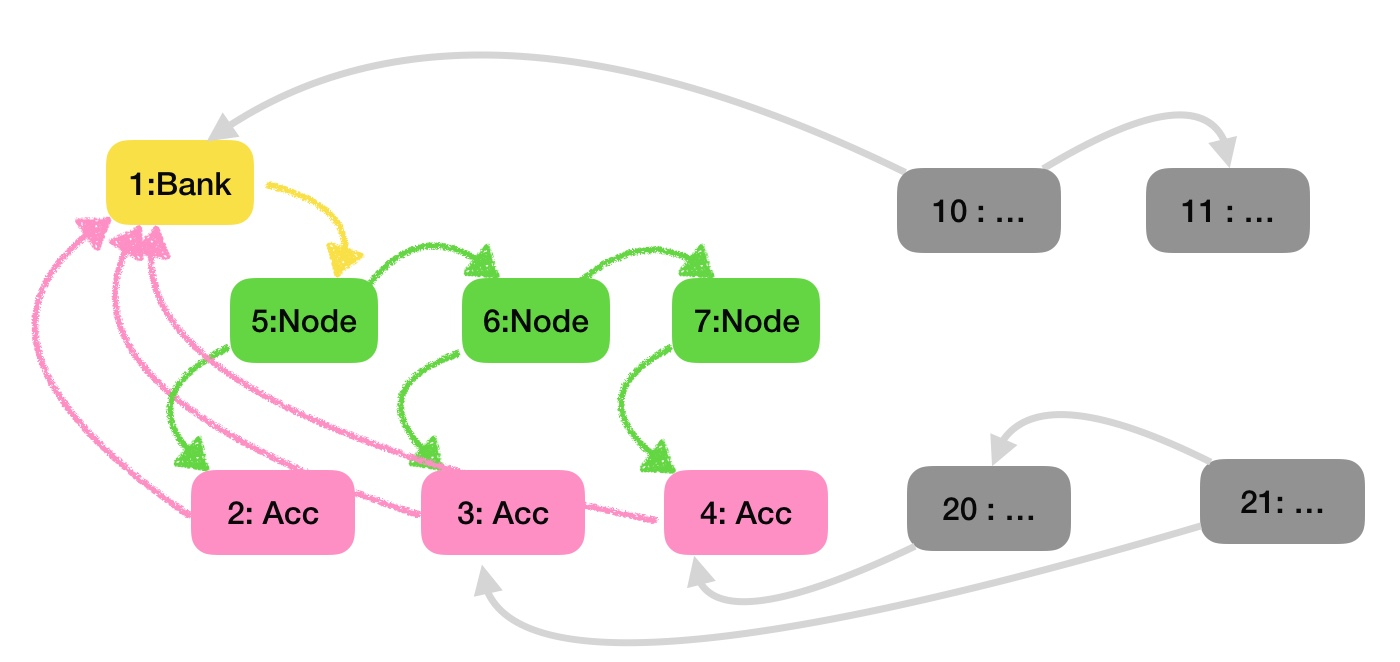
\includegraphics[width=11cm,height=5cm]{diagram1}
 \caption{Diagrammatic representation of some objects from  \prg{Bank}, \prg{Account} \etc  }
  \label{fig:Diagram}
  \end{figure}




\paragraph{Our Approach}
In order to specify robustness, we need to express
\begin{enumerate}
\item
access (permission) and  change (authority)
\item
{\em potential} effects (the future) and {\em causes} of effects (the past)
\item
footprints\footnote{use instead the tern footprint or witness?} (space) of executions as well as of assertions.
For example, an execution which starts (has as receiver) an object different than \prg{1}, and
 which involves objects
\prg{1}, \prg{2}, \prg{3}, \prg{4}, \prg{5}, \prg{6}, \prg{7}, \prg{20} and \prg{21},
might end up calling methods on \prg{1}, but is guaranteed not to affect the \prg{currency} on \prg{1}.

Interestingly, the temporal aspects of our assertions unify the footprint of an execution and an assertion\footnote{Better word?}: The foorprint of an assertion which talks about time is essentially the footprint of the execution involved in satisfying that assertion.
\end{enumerate}







\section{Our Proposal}

\subsection{Preliminaries}

Here we define some preliminaries ... they are more or less standard.\footnote{Most of the below can be taken from Swapsies work -- it is slightly simpler as we do not need $\obeys$}.
We will define the following:
\begin{enumerate}
\item
Runtime configuration $\sigma$; it consists of a heap, and a {\em rich} expression\footnote{Better term than "rich expression"?}. A rich expression consists of a stack of frames end expression contexts as well as the expression currently being executed. Explain that this is slightly unusual, but why it is useful
\item
A small OO PL with its syntax.
\item Also, syntax definitions for expressions $e$
\item
Also, syntax definitions for assertions $\A$.
\item
Modules $\M$:  a module maps a class identifier to a class definition; a function identifier to a function  and a predicate identifier to an assertion. A module concatenation operator,  $\M*\M'$ -- the operation is defined only when the
two modules do not have overlapping definitions.
\item
A small step operational semantics with the  format $\M, \sigma \leadsto \sigma'$
\item
an interpretation function for expressions $\interp{e}{\M,\sigma}$ which maps expressions and configurations to values.
\footnote{NOTE\_TO\_SELF: careful with undefinedness -- as per below for $\A$'s.
Also, we need to distinguish bad formedness because of infinite recursion
from undefinedness because of missing definitions.
We have all that in the Swapsies paper.}
\item
Define validity for assertions $\M, \sigma \models \A$. Eg the term
 $\prg{x}:\prg{C}$ expresses that $\interp {\prg{x} }{\M,\sigma}$ is the address of an object of class \prg{C};
\footnote{NOTE\_TO\_SELF: This is standard, but as we   allow for recursive efintions in $\M$ we also need to cater about infinite recursion and thus introduce undefinedness. In particular, if $\A \rightarrow \A'$, and if $\A$ undefined or  $\A$ is false but $\A'$ undefined? Ideally, these things have to be defined in such a way that usual manipulations hold, eg $\A \rightarrow \A' \ \equiv \neg A \vee \A'$.}
\item
Definition of the notion of initial configuration $\Initial{\_}$ and arising configuration $\Arising({\M})$. The   set  $\Arising(\M)$ contains all runtime configurations which can be reached
when starting with an empty heap,  and executing any expression consisting of constructor  and method calls
as defined in $\M$.\footnote{That is,
$\Arising(\M)$=$\{ \ \sigma\ \mid\ \exists \prg{e}.\ \M \vdash (\prg{e},\emptyset) \leadsto* \sigma \ \}$}

\end{enumerate}

\subsection{Extensions}

We will define the OCAP assertions $\CanAccess{\_}{\_}$  (permission)
and   $\Changes{\_}$ (authority). \footnote{Note that they are slightly different
assertions to those we had in the past.}
We also add temporal modifiers, where $\Future \A$ expresses that $\A$ will hold at some future point,
$\Past \A$ expresses that $\A$ held at some point in the past.
We also add a {\em spatial modifier}, $\Using{\A}{S}$, which expresses that assertion $\A$ holds in
the sub-configurations determined by the witness \prg{S}.

We extend the syntax for assertions as follows:\footnote{The symbols are not that good -- esp the symbols for future and past.}

\begin{definition}[Assertions]
$$\A ::=\  ... \mbox{as before} ...\ \ \mid \ \CanAccess x y \ \mid\  \ \Changes e \ \mid\  \Calls{m} \ \mid\  \\ \Future \A \ \mid \ \Using \A S  \ \mid \  \Past \A$$
\end{definition}



\begin{definition}[Time, Permission, Authority,  and Space ]
\label{def:permission}
Given a module $\M$, identifiers \code{x} and \code{y}, expression $\sE$, and runtime configuration $\sigma$, and a set of addresses $S$,
we define validity of the assertions   .... as follows:

\begin{itemize}
\item
$\Prog{},\sigma \models  \Future \A$\ \ iff\ \  $\exists \sigma'.\, [\ \ \M,\sigma \leadsto^* \sigma' \ \wedge \ \M,\sigma' [\overline{x \mapsto \sigma(x)}]\models \A, \mbox{ where } \overline{x}=Free(\A)\   ]$.
\item
$\Prog{},\sigma \models  \Past \A$\ \   iff\ \  $\exists \sigma_1,....\sigma_n, k\!\in\![1..n-1).\ [ \Initial {\sigma_1}\  \wedge\ \sigma_n=\sigma\ \wedge\ \forall i\!\in\![1..n).\ \M,\sigma_i\leadsto  \sigma_{i+1}  $\\
\strut \hspace{5.7cm} $\ \wedge \  \ \M,\sigma_k[\overline{x \mapsto \sigma(x)}]\models \A, \mbox{ where } \overline{x}=Free(\A)\  ]$.
\item
$\Prog{},\sigma \models   \CanAccess{\prg{x}}{\prg{y}}$   \ \ iff  \begin{itemize}
\item
$\sigma(x)$=$\sigma(y)$, or
\item
$\sigma(\prg{x},\prg{f})$=$\sigma(\prg{y})$  for some field \prg{f},  or
\item
$\sigma(\prg{this})$=$\sigma(\prg{x})$ and
  $\sigma(\prg{z})$=$\sigma(\prg{y})$,
  $\strut \hspace{0.1cm}$
for some some parameter of local variable \prg{z}.
 \end{itemize}
 \item
 $\Prog{},\sigma \models   \Changes{\prg{e}}$   \ \ iff \  \
 $\exists \sigma'.\, [\ \ \M,\sigma \leadsto \sigma' \ \wedge \interp{e}{\M,\sigma} \neq \interp{e}{\M,\sigma'}\ \ ]$


\item
 $\sigma\!\mid_S$ denotes a {\em restriction} of $\sigma$ to the objects from the set $S$. That is, the domain of
 the heap in $\sigma\mid_S$ is $S$, and otherwise,  $\sigma\mid_S$ is identical to $\sigma$. An example appears in figure \ref{fig:DiagramRestricted}.
 \item
$\M,\sigma  \models \Using{\A}{\prg{S}}$  \  \ iff \ \
  $ \M,\sigma\!\mid_S\, \models \A $, where   $S=\interp {\prg{S}} {\M,\sigma} $.
 \item
 $\M,\sigma  \models \Calls {m}$ \ \ iff \ \ the method call in the current frame in $\sigma$ is
 \prg{m}\footnote{We will express this precisely  when we have the full definition of $\sigma$}
\end{itemize}
\end{definition}

\begin{figure}[btph]
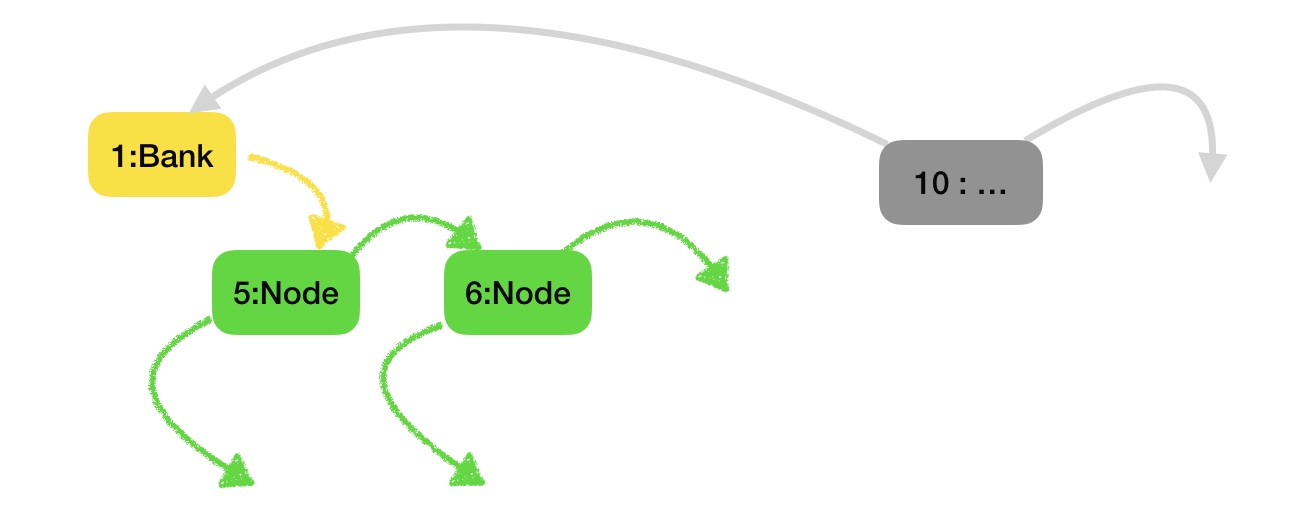
\includegraphics[width=10cm,height=4cm]{diagram2}
 \caption{Configuration from Fig. \ref{fig:Diagram} restricted to witness \{ \prg{1}, \prg{5}, \prg{6}, \prg{10} \}}
  \label{fig:DiagramRestricted}
  \end{figure}

Note that $\CanAccess{\prg{x}}{\prg{y}}$ is reflexive but  not transitive and not symmetric.

Also note the difference between $\Using{(\Future{\A})}{\prg{S}}$ and $\Future{(\Using{\A} }{\prg{S}})$.
For example,  the assertion  $\Using{(\Future{\prg{x}.\prg{f}=\prg{z}})}{\prg{S}}$ expresses that the current execution
leads to a future configuration  where
$\prg{x}.\prg{f}=\prg{z}$ will hold, and that the set \prg{S} suffices to witness this execution, while the assertion
$\Future{(\Using{{\prg{x}.\prg{f}=\prg{z}} }}{\prg{S}})$  expresses that the current execution
leads to a future configuration   where
$\prg{x}.\prg{f}=\prg{z}$ will hold and where  the set \prg{S} suffices to witness
that fact.
For example, take a configuration $\sigma$ where variable \prg{x} maps to some object \prg{31}, and where \prg{31} has a field \prg{f}
pointing to \prg{32}, and \prg{32} has a field \prg{f}
pointing to \prg{33}, and variable \prg{z} maps to  \prg{33}. Assume also that the expression to be executed in $\sigma$ starts with
\prg{x.f}=\prg{x.f.f}. Then we have that
$\M,\sigma  \models \Future{(\Using{{\prg{x}.\prg{f}=\prg{z}} }{\{\prg{x},\prg{z}\}})}$,
but
$\M,\sigma  \not\models \Using{(\Future{\prg{x}.\prg{f}=\prg{z}})}{\{\prg{x},\prg{z}\}}$.
On the other hand
$\M,\sigma  \not\models \Using{(\Future{\prg{x}.\prg{f}=\prg{z}})}{\{\prg{x},\prg{x}.\prg{f},\prg{z}\}}$

In general, for all $\M$ and $\sigma$, we have that
 $\M,\sigma \models  \Using{(\Future{\A})}{\prg{S}}$ implies $\M,\sigma \models \Future{(\Using{\A} }{\prg{S}})$, and that
 $\M,\sigma \models \Future{(\Using{\A} }{\prg{S}})$ implies that there exists a set $\prg{S}'$ such that
 $\M,\sigma \models  \Using{(\Future{\A})}{(\prg{S}\cup\prg{S'})}$.

\vspace{.2in}
We will prove that

\begin{lemma}[Preservation of validity and module linking]

$\M,\sigma \models \A$  \ \ \ then\ \ \ \   for all $\M'$ with $\M*\M'$ is defined:\ $\M*\M',\sigma \models \A$.
\end{lemma}




\subsection{Invariants}

We define below the meaning of invariants.\footnote{This part is as we had defined previously, with two simplifications: a) we do not need to worry about the $\obeys$-predicate here, and b) we do not distinguish the names of the classes and the names of participants in interfaces.}
The assertion $\M   \models\  \A$ requires that  the assertion $A$ is satisfied
in all reachable states.

\begin{definition}[Invariants]
\label{def:invariant}
\noindent
For a module $\M$  and assertion $\A$ we define:\\

 \begin{itemize}
 \item
$\M   \models\  \A$\ \ \  iff\ \ \ \
% $\strut\SP\SP$
$\forall \M'.\, \forall \sigma\!\in\!\Arising(\M'*\M).\ \M'*\M,\sigma \models \  \A$
 \end{itemize}
\end{definition}

The use of the set of configurations from $\Arising(\M'*\M)$ reflects that policies
 need to hold in an {\em open} world, where
we link against {\em any} module $\M'$,
about which we know nothing.

\subsection{Implication and equivalence}

\begin{definition}
\label{def:impl:equiv}
\noindent
For a module $\M$  and assertions $\A$  and $\A'$, we define strong equivalence and implication ($\equiv$ and $\sqsubseteq$), as well
as   weak equivalence and implication ($\approxeq$ and $\weakImplies$)  as follows:


 \begin{itemize}
\item
$\M   \models\  \A \strongImplies \A'$  \ \ \ \ iff \ \ \ \
$\forall \M'.\, \forall \sigma\!\in\!\Arising(\M'*\M).[\ \ \  \M'*\M, \sigma \models \A \  \ \  \longrightarrow\  \ \  \M'*\M, \sigma \models \A'\ \ \ ]$
 \item
$\M   \models\  \A \equiv \A'$ \ \ \ \ iff \ \ \ \
$\M   \models\  \A \strongImplies \A'\ \  \wedge \ \  \M   \models\  \A' \strongImplies \A$
%$\forall \M'.\, \forall \sigma\!\in\!\Arising(\M'*\M):\ \ \  \M'*\M, \sigma \models \A \  \ \longleftrightarrow\   \ \M'*\M, \sigma \models \A'$
\item
$\M   \models\   \A \weakImplies \A'$  \ \ \ \ iff \\ \ \ \ \ \ \
\strut  \hspace{1cm}  $\forall \M'.\, \forall \sigma\!\in\!\Arising(\M'*\M).\,\M'*\M, \sigma \models \A$ \  \ \  $\longrightarrow$\  \ \
$\forall \M'.\, \forall \sigma\!\in\!\Arising(\M'*\M).\,\M'*\M, \sigma \models \A'$
\item
$\M   \models\  \A \approxeq \A'$   \ \ \ \ iff \ \ \ \ \
$ \M  \models  \A \weakImplies \A' \   \ \wedge\   \  \M  \models  \A' \weakImplies \A$
 \end{itemize}
\end{definition}

The definitions from above are applicable to the empty module, eg  $\models\  \A \equiv \A'$ iff   all modules $\M$ satisfy $\M \models\  \A \equiv \A'$.
The following properties hold:

\begin{lemma}
For all modules \M, assertions \A and \A':

 \begin{itemize}
 \item
$\M   \models\  \A \equiv \A'$  \ \ \ implies \ \ \  $\M   \models\  \A \simeq \A'$
\item
$\M   \models\  \A \strongImplies \A'$  \ \ \ \ implies  \ \ \ \
$\M \models \A \weakImplies \A$
\item
$\M \models   \Using{(\Future{\A})}{\prg{S}}\ \strongImplies\ \Future{(\Using{\A} }{\prg{S}})$
\item
$ \M \models\  \Future{\A}\rightarrow \A' \  \  \weakImplies \ \ \A\rightarrow\Past{\A'}$
 \end{itemize}
\end{lemma}

\paragraph{Space-Monotonicity}\footnote{Not sure how useful this concept is}

\begin{definition}[Space-Monotonicity]
We call an assertion $\A$ {\em space-monotonic} in $\M$, iff for all set expressions $\prg{S}$ and  $\prg{S}'$,
  % $\M,\sigma\models ( \prg{S} \subseteq \prg{S}'\ \wedge\  \Using{\A, \prg{S}}) \ \strongImplies\  (\Using{\A, \prg{S'}})$
%\end{definition}\footnote{If we unfold the definitions, we obtain that
% $\A$ is space-monotonic in $\M$, iff for all set expressions $\prg{S}$ and  $\prg{S}'$
 and all $\sigma\in\Arising({\M})$:
 \\
  If  $\M,\sigma\models  \prg{S} \subseteq \prg{S}'$ and $\M,\sigma\models  \Using{\A} {\prg{S}}$, then
$\M,\sigma\models  \Using{\A}{ \prg{S'}}$
\end{definition}

We prove space monotonicity for some assertions

\begin{lemma}[Space-Monotonicity for change and access]
$ ~ $

\begin{itemize}
\item
${\Changes \sE} $ is space-monotonic.
\item
$\CanAccess {\prg{x}}{\prg{y}}$ is space-monotonic.

\end{itemize}
\end{lemma}

Not all assertions  are not space-monotonic. E.g. $\forall a:\prg{Account}.\prg{a.balance}\geq 3$ is not space-monotonic.


The following lemma would be nice to have -- otherwise we will need to change the definition of monotonicity.

\begin{lemma}[Space-Monotonicity and module linking]
If $\A$ is space-monotonic with $\M$, then it is also space-monotonic with $\M*\M'$.
\end{lemma}


 \section{Specifications for Robustness Policies}

 We now use the concepts introduced in the earlier sections to specify various robustness policies

 \subsection{Specification of \Pol 2  and   \Pol 4}

We    give a formal definition of \Pol 2 and  \Pol 4, using the concepts defined earlier in  Definition \ref{def:permission}: %

\begin{definition}
\label{def:pol2}
We define  what it means for an object \prg{o} to be internal to a bank's data structure, an then define \Pol 2  and   \Pol 4  as follows:

%  \noindent
$\prg{Internal}(\prg{b})$ \ \  $\triangleq$ \ \
$\{\ \prg{o}\ \mid\  \prg{b}:\prg{Bank}\ \ \wedge \ \ (\ \prg{o} = \prg{b}\ \ \vee\  \ \prg{o}:\prg{Account}\wedge \prg{o}.\prg{myBank}=\prg{b}$\\
\strut \hspace{7.3cm} $\ \ \vee\ \ \ \exists k. \ \prg{b}.\prg{ledger}.\prg{next}^k = \prg{b})\ \ \ \ \}$


$\prg{Internal}'(\prg{a})$ \ \  $\triangleq$ \ \
$\{\ \prg{o}\ \mid\  \prg{a}:\prg{Account}\ \ \wedge \ \
 \prg{a}.\prg{myBank} :\prg{Bank}\ \wedge\  \prg{o}\in \prg{Internal}(\prg{b})\ \}$


 \vspace{.2cm}

  \Pol 2\ \  $\triangleq$ \ \
  $\forall \prg{b}.\forall \prg{S}.
  [ \ \  \prg{b}:
  \prg{Bank}\ \wedge\ \prg{this}\neq\prg{b}\ \wedge\ \ \Using{(\Future\Changes{\prg{b.currency}})}{\prg{S}} \ \ \ \ \longrightarrow \ \  $\\
   \strut $~ $ \ \ \ \hspace{1.7in}  \hfill
 $\exists \prg{o}. \ [ \ \
  \prg{o}\in \prg{S}\   \wedge\  \CanAccess{\prg{o}}{\prg{b}}\ \wedge\     \prg{o}\notin\prg{Internal}(\prg{b})  \ \ ]\ \ ]$


 \vspace{.1cm}
% \noindent
    \Pol 4\ \  $\triangleq$\ \ $\forall \prg{a}.\forall \prg{S}.\ [ \ \  \prg{a}:\prg{Account}\   \wedge\   \prg{this}\neq\prg{a} \ \wedge\ \Using{(\Future\Changes{\prg{a.balance}})}{\prg{S}}\ \ \   \
    \longrightarrow$ \\
 $\strut \hspace{3.9cm} \hfill \exists \prg{o}.\ [\, \prg{o}\in \prg{S}\ \wedge \ \CanAccess{\prg{o}}{\prg{a}}\ \wedge  \ \prg{o} \notin\prg{Internal}'(\prg{a}) \ ] \ \ \ \ ]$

\end{definition}

\paragraph{Discussion}
In other words, \Pol 2  mandates that the elements of the data structure (ie the elements from $\prg{Internal}(\prg{b})$) cannot be used (are not sufficient) to  change the currency of the bank. If a computation takes place inside the set \prg{S}, and {\em in the current state} in \prg{S}
all accesses to the bank go through elements of the data structure (ie the \prg{Account} objects),\footnote{Say why we can ignore \prg{Node} objects} then we have a guarantee that the computation will not affect the currency.
For example, if a computation takes place in the context of objects \prg{1}, \prg{2}, \prg{3}, \prg{4}, \prg{5}, \prg{7}, \prg{20} and \prg{21}, and the current receiver is no \prg{1}, then we have a guarantee that the currency of \prg{1} will not be affected. So, even through \prg{1} is involved in the computation, because there is no {\em external} access to it, we have a guaratee that the method \prg{makeAccount} will not be called on it.

An alternative way of expressing \Pol 2 is as follows:


 \Pol 2\ \  $\equiv$ \ \
  $\forall \prg{b}.\forall \prg{S}.
  [ \ \  \prg{b}:
  \prg{Bank}\ \wedge\   \prg{b}\neq\prg{this}\ \wedge\  \forall \prg{o} \in \prg{S}.\, [\ \prg{o}\in\prg{Internal}(\prg{b}) \ \vee\  \neg  \CanAccess{\prg{o}}{\prg{a}}  \ \ ]$
\\ \hfill \strut $~   \ \ \ \hspace{1.7in}  \  \ \longrightarrow \ \ \ \neg(
 \Using{(\Future\Changes{\prg{b.currency}})}{\prg{S}})\   \  \ \ ]$

\vspace{.01in}
% TO\_DO: discuss the difference between  $\Using{(\Future\Changes{\prg{b.currency}})}{\prg{S}})$, and
% $\Future{(\Using{\Changes{\prg{b.currency}}{\prg{S}})}}$.

\vspace{.01in}
\Pol 2  guarantees
that if an object \prg{o}$\neq$\prg{b} may affect the value of \prg{b.Currency} only if the  objects
involved in the process of affecting the value of \prg{b.Currency}  include at least an object $\prg{o}'$
which had direct access to \prg{b}, and
whose class is  not  \prg{Account}. Stated positively, this policy mandates
that exporting an \prg{Account} to an environment will not affect the \prg{Currency} of \prg{b}.
In other words,
\prg{Account}s protect the integrity of the \prg{Bank}'s currency.


In more detail, by applying  Definition \ref{def:invariant} on Definition \ref{def:pol2}, the  meaning of policy \Pol 2
  is, that a runtime configuration $\sigma$ satisfies  \Pol 2  if whenever the current receiver in $\sigma$
 is not a \prg{Bank} object, and the execution of $\sigma$ leads to another runtime configuration $\sigma'$
 with a different value for \prg{b.Currency}, then the objects involved in the execution from
 $\sigma$ to $\sigma'$ include at least one object which had direct access to \prg{b}.
 Note that this direct access needs to exist at the beginning of   the execution, \ie at $\sigma$.
 Formally:

 \noindent
 $\M, \sigma \models  \Pol 2$\\$ \strut \ \ \ \  \ \  \longleftrightarrow $\\
 $\forall \prg{b}.\forall S.\ [ \ \ \ \ \M, \sigma \models \prg{b}:\prg{Bank}\ \wedge\
 \sigma(\prg{b})\neq \ \sigma(\prg{this}) $\\
 $\strut \hspace{2.1cm}  \wedge \
 \ \exists\sigma'.(\ \ \ \ \M, \sigma\mid_S \leadsto^* \sigma'\
\ \wedge\ \interp {\prg{b.Currency}}{\M,\sigma}\neq \interp {\prg{b.Currency}}{\M,\sigma'[\prg{b}\mapsto\sigma(\prg{b})]}\ )$\\
$\strut \hspace{4.7cm} \longrightarrow$ \\
 $\strut \hspace{2.7cm}  %\exists \prg{o}. (\ \  \sigma(\prg{o}) \!\!\in\!\!\prg{S}\ \
 \exists \prg{o}. (\ \ \prg{o} \!\in\!S\ \
  \wedge \ \ \M, \sigma \models \CanAccess{\prg{o}}{\prg{b} }\ \wedge \  \prg{o}\notin \prg{Internal}(\prg{b}) \   \ ) \ \ \ \ \ \ \  ]$



\subsection{Specifying  "no leaks"}

This is a family of guarantees that Dean seemed especially interested in, when we discussed in March in London.
For the particular example, we want to express that

\begin{description}
\item[\Pol 7]
The \prg{Bank} does not leak out of the \prg{Bank}/\prg{Account} system
%\item[Pol\_7]
%The \prg{Accounts} do  not leak out of the \prg{Bank}/\prg{Account} system
\end{description}

And we give a formal specification

\begin{definition}[Banks do not leak]
\label{def:bankNoLEak} We define \Pol 7 as follows:

\Pol{7}\ \  $\triangleq$\ \ $\forall \prg{b}.\forall \prg{S}.\ [  \ \ \prg{b}:\prg{Bank}\ \wedge\  \prg{o}:\prg{Object}\  \wedge\   \neg(\CanAccess{\prg{o}}{ \prg{b}})\ \wedge\   \Using {(\Future{\CanAccess {\prg{o}}{\prg{b}}})} {\prg{S}} $
 \\  $\strut$ \hspace{4cm}
  $\longrightarrow$
 $\strut \hspace{0.5cm}  \exists \prg{o}'.\ [\, \prg{o}'\in \prg{S}\ \wedge \  \CanAccess{\prg{o}'}{ \prg{b} }\ \wedge\   \prg{o}' \notin \prg{Internal}(\prg{b}) \, ) \ ] \  \  \ \  ]$

%\hspace{.1cm}
%{\bf {Pol\_8}}\ \  $\equiv$\ \ $\forall \prg{o},\prg{b}, \prg{o}'\forall \prg{S}.\ [  \ \ \prg{b}:\prg{Bank}\ \wedge \prg{o}\in\prg{Internal}({\prg{b}})\ \wedge\  \prg{o}':\prg{Object}\ \ \neg(\CanAccess{\prg{o}'}{ \prg{o}})\ \wedge\   \Using {(\Future{\CanAccess {\prg{o}'}{\prg{o}}})} {\prg{S}} $
% \\  $\strut$ \hspace{4cm}
%  $\longrightarrow$
% $\strut \hspace{0.5cm}  \exists \prg{o}''.\ [\, \prg{o}''\in \prg{S}\ \wedge \  \CanAccess{\prg{o}''}{ \prg{o} }\ \wedge\   \prg{o}'' \notin \prg{Internal}(\prg{b}) \, ) \ ] \  \  \ \  ]$
\end{definition}

In other words, \Pol 7 guarantees that objects that are internal to the bank \prg{b} do not leak access to it.
In more detail: if   objects  \prg{o} and \prg{b} exist  now, and \prg{o} does not have direct access to \prg{b} now, but obtains
access to \prg{b} through some computation which involves objects from the set \prg{S}, then at least one  object  from \prg{S} has
now direct access to   \prg{b} and this object is not internal to \prg{b}.

\section{Adherence to Policies}
\label{section:Adherence}
In this section we will outline the proofs that particular modules adhere to their specifications.
This serves to demonstrate the practicality of our approach.
In particular we will show two different versions fo the \prg{Bank}/\prg{Account} example (sections \ref{section:Adherence:ModuleOne} and \ref{section:Adherence:ModuleTwo}, and we will prove that
both satisfy the policies \Pol 2, \Pol 4, and \Pol 7, while they differ in the definition of \prg{Internal}.
But before doing that, in section \ref{section:GeneralPropertiesExecution}, we will study some further properties of execution.


\subsection{General properties of execution}\footnote{Find better title?}
\label{section:GeneralPropertiesExecution}

We will first define some further predicates which reflect over the program execution and prove
some general properties of program execution.

We call a locations set, \prg{L}, an expression which denotes a set of addresses and field identifiers, \eg, $\{\ (\prg{b},\prg{ledger}), (\prg{b}.\prg{ledger},\prg{balance})\ \}$ is such a locations set.

\begin{definition}[Framing]
Take arbitrary module \M, assertion \A, , ...

\begin{itemize}
\item
\interp{\prg{L}}{\sigma,\M*\M'} = ....
\item
$ \sigma\mid _L$ ....
\item
$\M, \sigma \models \prg{L} \frames \prg{e}$\ \ \ \  \ iff \ \ \ \ \
$\forall \M'.\forall \sigma'\!\in\!\Arising({\M*\M'}). \forall L.$\\
\strut \hspace{1cm} $  [ \ \ L=\interp{\prg{L}}{\M,\sigma}\, \wedge\,
 \sigma\mid _L= \sigma'\mid_L \ \   \longrightarrow\ \ \   \interp {\prg{e}}{\sigma,\M*\M'}  =  \interp {\prg{e}}{\sigma',\M*\M'}
\ \ ]$
\item
$\M  \models \prg{L} \frames \prg{e}$\ \ \ \  \ iff \ \ \ \ \
$\forall \M'.\forall \sigma\!\in\!\Arising({\M*\M'}). \ \M'*\M, \sigma \models \prg{L} \frames \prg{e}$
\item
$\M, \sigma \models \prg{L} \frames\A $\ \ \ \  \ iff \ \ \ \ \
$\forall \M'.\forall \sigma'\!\in\!\Arising({\M*\M'}). \forall L.$\\
\strut \hspace{1cm} $ [ \ \ L=\interp{\prg{L}}{\M,\sigma}\, \wedge\,
\sigma\mid _L= \sigma'\mid_L \ \   \longrightarrow\ \ \   [\ \M*\M',\sigma \models \A   \ \longleftrightarrow\ \M*\M',\sigma' \models \A
\ \ ] $
\item
$\M  \models \prg{L} \frames \A$\ \ \ \  \ iff \ \ \ \ \
$\forall \M'.\forall \sigma\!\in\!\Arising({\M*\M'}). \ \M'*\M, \sigma \models \prg{L} \frames \A$
\end{itemize}

\end{definition}

NOTE\_TO\_SELF: we need to think about whether we also need to make \prg{L} self-framing.
Also, rethink whether we need to stick new modules $\M'$ to the whole thing.
--
Also, the sets are not equal -- they are isomorphic. We can deal with isomorphisms, but
it has a high notation penalty. Can we pretend that they are equal? hmhhhhh


And then we can prove that changes in the interpretation or the validity require a change in the frame:

\begin{lemma}[Change in the context of framing]
Take arbitrary module \M, assertion \A, such that  $\sigma\in\Arising({\M*\M'})$

\begin{itemize}
\item
If  $\M  \models \prg{L} \frames \prg{e}$, and
$\M'*\M, \sigma \models \Using{(\Future{\Changes{\prg{e}}})}{\prg{S}}$, \\
then there exists a pair $(\prg{e}',\prg{f})$ , with
$\M,\sigma \models (\prg{e}',\prg{f})\in \prg{L}$\footnote{Sophia, you need to check this bit  what if \prg{z}
there is no handle in \prg{L}, eg what if \prg{L} talks about anonymous objects
\eg \prg{L} = $\{ o \ \mid o.\prg{myBank}=\prg{b} \}$?Here $o$ is anonymous. Also, do we need $\M$ or $\M'*\M$?}
and $\M'*\M, \sigma \models  \Using{\Future{\Changes{\prg{e}'.\prg{f}}}}{\prg{S}}$

\item
similar for
$\M'*\M, \sigma \models \Using{\Future{\Changes{\A}}}{\prg{S}}$
\end{itemize}

\end{lemma}

\begin{figure}[tbp]
\begin{lstlisting}
 class Bank {
   private field ledger;   // a Node

   Bank( )
     { ledger = null; }
   fun makeAccount(amt)
     { account = new Account(this);
       ledger = new Node(account, amt, ledger);
       return account; }
   fun deposit(source, destination, amnt)
     { sourceNd = ledger.getNode(source)
       destinationNd = ledger.getNode(destination)
       if (sourceNd!=null && destinationNd!=null && sourceNd.balance>amt) then
          { < sourceNd.balance = sourceNd.balance-amt
              destinationNd.balance = destinationNd.balance+amt > }
        else
          { return }               }
 }

 class Account {
   private field myBank;  // a Bank

   Account(aBank)
     { myBank = aBank;  }
   fun sprout( )
     // create Account in same Bank with 0 balance
     { return this.myBank.makeAccount(0)  }
   fun deposit(source, amnt)
     // if destination is an Account in myBank,  and  source holds enough money,
     // then transfer amnt from source into receiver
     { myBank.deposit(source,this,amnt) }
 }

  class Node{
   field balance;     // the  money held in theAccount a number
   field next;        // the next node
   field theAccount;  // the account

   fun getNode(account)
     { if (theAccount==account) then
           { return this }
       elseif (next!=null)
           { next.getNode(account) }
       else
           {  return null }            }	
 }
\end{lstlisting}
\caption{\MOne: First version of the Bank example, in detail}
\label{fig:BankDetailedOne}
 \end{figure}


We now think a bit more about changes in accessibility. The predicate  $\Gives(\prg{x},\prg{y},\prg{z})$ expresses
that \prg{x} passed to \prg{y} access to \prg{z}.

\begin{definition}[Giving]
For arbitrary module \M and $\sigma$, we define:

\begin{itemize}
\item
$\M,\sigma  \models \Gives(\prg{x},\prg{y},\prg{z})$\ \ iff \ \
$\sigma(\prg{this})$=$\sigma(\prg{x})$ \  $\wedge$ \
$\M, \sigma \models \neg (\MayAccess( \prg{y},\prg{z})\,)$ \ $\wedge$ \\
\strut \hspace{.9cm} $\exists \sigma'. \ [\  \M,\sigma \leadsto \sigma'  \  \wedge  \
 \M,\sigma' \models \MayAccess( \prg{y},\prg{z})\ ]$
\end{itemize}

\end{definition}

The following lemma says that any changes in accessibility witnessed\footnote{is that the right term? or frames?}
by set \prg{S} is due to an element of \prg{S} giving the object.

\begin{lemma}[Change in Accessibility is caused by Giving]
For any module \M, and  $\sigma$

\begin{itemize}
\item
If  $\M, \sigma  \models \neg(\MayAccess(\prg{y},\prg{z}))$, and
$\M, \sigma \models \Using{(\Future \MayAccess(\prg{y},\prg{z}))}{\prg{S}}$, \\
 then there exists a  $\prg{x}$  and  $\prg{y}'$, with
%$\M,\sigma \models  \prg{e} \in \prg{S}$, and
$\M,\sigma \models \Using{(\Future{\Gives(\prg{x},\prg{y}',\prg{z})})}{\prg{S}}$.
\end{itemize}

\end{lemma}

\subsection{Adherence to Policies for module \MOne}
\label{section:Adherence:ModuleOne}

In figure \ref{fig:BankDetailedOne} we show the  code for \MOne in detail.

\subsubsection{\MOne~preliminaries}
We define the footprint of \prg{b.balance} as

\begin{definition}We define the currency-footprint of a bank as follows:

$\prg{CurrencyFootprint}(\prg{b})$ $\triangleq$
$\{ \ (\prg{b},\prg{ledger}) \} \ \cup$\\
\strut \hspace{4.8cm}
$\{ \ (\prg{o},\prg{balance})\ \mid \exists k:\mathbb{N}. \prg{x}.\prg{ledger}.\prg{next}^k=\prg{o} \ \}$
\end{definition}

\begin{lemma}
$\MOne \models \prg{b}:\prg{Bank} \rightarrow \prg{CurrencyFootprint}(\prg{b}) \frames \prg{b}.\prg{currency}$
\end{lemma}

We also define a predicate $Gives(prg{x},prg{y},prg{z})$ which expresses that while \prg{x} was excuting, it
passed to \prg{y} access to \prg{z}.
... more in handwritten notes ...

\subsubsection{\MOne~adheres to \Pol 2}
\begin{lemma}
$\MOne \models \Pol 2$
\end{lemma}
Proof sketch   in Sophia's handwritten notes.

\subsubsection{\MOne~adheres to \Pol 4}

\begin{lemma}
$\MOne \models \Pol 4$
\end{lemma}

\subsubsection{\MOne~adheres to \Pol 7}

\begin{lemma}
$\MOne \models \Pol 7$
\end{lemma}
Proof sketch  in Toby's handwritten notes.

\subsection{Adherence to Policies for module \MTwo}
\label{section:Adherence:ModuleTwo}

In figure \ref{fig:BankDetailedTwo} we show the  code for \MTwo in detail.

\begin{figure}[tbp]
\begin{lstlisting}
 class Bank {    }

 class Account {
   protected field balance; // the data of the Account;
   protected field myBank;  // a Bank

   Account(aBank,amt){
     balance = amt;
     myBank = aBank }

   fun deposit(source, amnt){
     if ( myBank== source.myBank && source.balance>=amt && amt>0) then
        { source.balance = source.balance-amt;
           this.balance = this.balance + amt }    }
}

\end{lstlisting}
\caption{\MTwo: Second version of the Bank example, in detail}
\label{fig:BankDetailedTwo}
 \end{figure}

We give the code for \MTwo~ in Figure ???, and define \prg{Internal} as follows.
The code works through ...
The set  \prg{Internal} describes ....


\subsubsection{\MTwo~adheres to \Pol 2}

\subsubsection{\MTwo~adheres to \Pol 4}

\subsubsection{\MTwo~adheres to \Pol 7}


\section{Hoare Logic}
\label{section:Hoare}
Here we give Hoare Logic rules which allow us to prove adherence to policies.
NOTE: Not sure when we will get to do these rules. If we get to define these rules, then we will use them for the proofs
 in section \ref{section:Adherence:ModuleOne}
and we will swap section \ref{section:Adherence} and section \ref{section:Hoare}

\section{Further Applications}
In this section we will apply our methodology to give specifications to other famous patterns from the OCAP literature,
\ie the membrane, the DOC-tree, and ...

\subsection{The DOM tree}
....

\subsection{The membrane}
...

\subsection{Sealer/Unsealer}

In Figure \ref{fig:WrapUnwrap} we visit the sealer/unsealer example  from cite-Morrison and Miller.


\begin{figure}[tbp]
\begin{lstlisting}
 class Box{
   ...
   fun seal(element){... }
   fun unseal(sealed){ ... }
 }

\end{lstlisting}
\caption{Wrapping and Unwrappingl}
\label{fig:WrapUnwrap}
 \end{figure}

The specification of these functions mandates \prg{seal} wraps the object into another structure, and \prg{unseal} unwraps the original object out of the structure, Like cite(David Swasey, OOPLSA'13), we use an uninterpreted  predixate, $\prg{Wrapped}(\prg{z},\prg{o},\prg{b})$ which expresses that \prg{z} contains the value of \prg{o} as wrapped by \prg{b}.

The policies from below express that \prg{seal} wraps an object, while \prg{unseal} unwraps it, and they are very similar to those from cite(David Swasey, OOPLSA'13).

\Pol {seal\_1} $\triangleq$
\strut \hspace{2.1cm} $\prg{o}:\prg{Object}\ \wedge\ \prg{b}:\prg{Box}$  \\
\strut \hspace{6cm}$\{\ \prg{x} = \prg{b}.\prg{seal}\prg{(o)}\ \}$\\
\strut \hspace{5cm} $\prg{Wrapped}(\prg{x},\prg{o},\prg{b})$

\hspace{.1cm}

\Pol {seal\_2} $\triangleq$
\strut \hspace{2.2cm}$\prg{o}:\prg{Object}\ \wedge\ \prg{b}:\prg{Box}\  \wedge\  \prg{Wrapped}(\prg{x},\prg{o},\prg{b})$\\
\strut \hspace{6cm}$ \{\ \prg{y} = \prg{b}.\prg{unseal}\prg{(x)} \}$\\
\strut \hspace{5cm} $\prg{y}=\prg{o}$

\hspace{.1cm}

But further to the specification from cite(David Swasey, OOPLSA'13) ,
we want to also express that the {\em only} way to extract a sealed object
 out of its box, is by calling the \prg{unseal} function on the box. For this, we
 define an assertion $\prg{Sealed}(\prg{o})$ which expresses that {\em all} accesses to \prg{o}
go through some sealed box, and the assertion $\prg{UnSealed}(\prg{o})$ which expresses that the object can be accessed without
going through a sealed box. Using these predicates, in  \Pol {seal\_3} we express that if a sealed object
becomes unsealed, then this must have happened though a call to the \prg{unseal} function:



$\prg{Sealed}(\prg{o}) \  \triangleq\ \prg{o}:\prg{Object}\ \wedge$\\
\strut \hspace{2.75cm}$ \forall \prg{o}':\prg{Object}.\ [ \ \CanAccess{\prg{o}}{\prg{o}'}\ \wedge \prg{o}\neq\prg{o'}\ \rightarrow\ \exists \prg{b}:\prg{Box}.\prg{Wrapped}(\prg{o}',\prg{o},\prg{b})\ ]$

$\prg{Unsealed}(\prg{o}) \  \triangleq\ \neg \prg{Sealed}(prg{o})$

\hspace{.05cm}

\Pol {seal\_3} $\triangleq$  $\forall \prg{o}.\forall{\prg{S}}.$ \ \
% $\\ \strut \hspace{4cm} $
$[\ \ \Using{(\, \prg{Sealed}(\prg{o}) \ \wedge\ {\Future{\prg{Unsealed}({\prg{o}})}}\, )}{\prg{S}} \ \ \ \longrightarrow $\\
\strut \hspace{8cm}$ \exists \prg{b},\prg{x}.[ \prg{b},\prg{x}\in\!\prg{S}\ \wedge\   \prg{Wrapped}(\prg{x},\prg{o},\prg{b}) \ \wedge$\\
\strut \hspace{9cm}$\Using{(\Future{\Calls{\prg{b.unseal}(\prg{x})}})}{\prg{S}}\ ]
$\footnote{This definition is not perfect, as it does not preclude that the call to $\prg{b.unseal}(\prg{x})$ could happen {\em after}
\prg{o} became \prg{Unsealed}. Perhaps, we should instead have an assertion combinator ${\A\, \kw{to} \A'\,\kw{caused by} \prg{code}}$, and we could then say:

\Pol {seal\_3} $\triangleq$  $\forall \prg{o}.\forall{\prg{S}}.$ \ \
% $\\ \strut \hspace{4cm} $
$[\ \ (\Using{{\prg{Sealed}(\prg{o})}}{\prg{S}}) \  \kw{to}\  (\Using{\prg{Unsealed}({\prg{o}})}{\prg{S}})\ \kw{caused\,by}\  \prg{b.unseal}{(\prg{x})} \ ]$
}




\subsection{The DAO }

We describe here only some aspects of the DAO contract.
The DAO keeps a table called \prg{balances} which keeps track of the balances for all its clients.
 The following three policies mandate that \Pol {DAO\_1}: the contents of \prg{o.balances} can only be affected by \prg{o}
 itself, that \Pol {DAO\_2}: the ether held in the DAO is the sum of the balances in all its participants, and \Pol {DAO\_3}: that any
 participant can withdraw up to amount that the the DAO holds for it.
 In fact, with \Pol {DAO\_2} is too strong, \Pol {DAO\_1} and \Pol {DAO\_3} are not, and any
 contract adhering to these two policies would have not suffered from the DAO-attack\cite{...}.


In the below we also have the use a lookup function $\Caller$ with obvious meaning\footnote{we can define it with what we have}.

~ \\
\noindent
$\Pol {DAO\_1}$ $\triangleq$ $ ...\ \Changes{\prg{dao.balances(o)}}\  \longrightarrow\   \Caller=\prg{o} ....$

~ \\
\noindent
$\Pol {DAO\_2}$ $\triangleq$ $ ... \prg{dao.ether}=\sum_{o\in dom(\prg{dao.balances})}  \prg{dao.balances(o)}$

~ \\
\noindent
$\Pol {DAO\_3}$ $\triangleq$ $... \ \prg{dao.balances(o)}=m \ \wedge\ \Caller = \prg{o}\ \wedge\ \Calls{payme} \ \wedge\ \prg{x}=m'\leq m  \longrightarrow  $\\
\strut \hspace{5cm}
$\Future{(\Caller=\prg{dao}\ \wedge\ \Calls{send} \ \wedge\  \prg{x}=m')}$\footnote{SOPHIA: Here is a point where we
want the parameters to have the meanings as in the future configuration! Easy to fix- stick in the calls names for the arguments}

Note that $\Pol {DAO\_3}$ is a liveness property. It promises that if one of the \prg{DAO} participants asks to be paid back
(by calling \prg{payMe}), then eventually they will get their money back (in the future the \prg{DAO} will call the function \prg{send}
with the appropriate ether argument).


\section{Discussion}
In this section we compare ``classical'' specifications with those proposed here\footnote{shall we call them ``holistic''?}

\begin{itemize}
\item Classical specifications reflect over (\ie mandate properties of) the state of the execution now, while
holistic specifications can also reflect over the possible  states   reachable from now, or those states in the past
which lead to the current state.

\item Classical specifications describe what happens under {\em correct} use  of the data structure,
while holistic specifications  describe preservation of properties under {\em arbitrary} use  of the data structure.

\item Both specifications employ notions of footprint\footnote{In separation logic, and also others}, but
classical footprints are related to the carrier set\footnote{Witness??} of properties in the current state, while
because  of the temporal operators  of holistic specs, holistic witnesses\footnote{not sure whether witness of footprints}
 can  also talk about the carrier sets\footnote{Witness??} of arbitrary executions.
 Also, holistic witnesses are first order\footnote{I expect that in some sep logic they are first order too, but perhaps we
 can compare with the first version of sep logic}

% \item Classical specifications describe the effects of code execution, while holistic specs also reflect over
 %describe the causes of -- this is related to the next item
%  arbitrary effects, such as $\Future{\Changes{\prg{e}}}$.


\item Classical specifications describe sufficient conditions, while holistic specifications also describe necessary conditions. 
Namely, the assertion  $\A \rightarrow \Future{\A'}$ says that $\A$ is a {\em sufficient} condition to achieve the
effect $\A'$ in the future, while $(\Future{\A'}) \rightarrow \A$ says that $\A$ is a {\em necessary} condition to achieve $\A'$ in the future.

\item Defensive Programming Rather than
      "What can the others (client) achieve using my code"
Say
     "What do I prevent the others from doing with my objects"

 \item
 From KVM paper: From the KVM paper

"Contract interactions are often complex, with safe contracts able to have their guarantees violated by calling into potentially malicious and unknown third party contract code."

Rather than say
    What can the others expect from me
We say
    What do I have to make sure the others cannot do with my objects

Elias
    Modularity is the ability to ...

    In order to deduce that xxx I must lookat the spec of yyy methods/

    Has modular verif gone too far?

Modular verification should not imply modular specifications

\end{itemize}




\section*{Bibliography}
 \bibliographystyle{plain}
 \bibliography{Case}



\end{document}

